\begin{exo}
	On tire une boule dans une urne dont le contenu est illustré ci-dessous.
	\begin{center}
		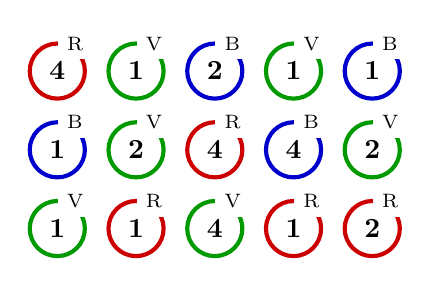
\begin{tikzpicture}
			\draw[red!80!black, line width=1.5pt] (0,0) circle (0.35); \node[above=-0.5mm, right,fill=white] at (0, 0.4) {\scriptsize R}; \node at (0,0) {\textbf{4}};
			\draw[green!60!black, line width=1.5pt] (1,0) circle (0.35); \node[above=-0.5mm, right,fill=white] at (1, 0.4) {\scriptsize V}; \node at (1,0) {\textbf{1}};
			\draw[blue!80!black, line width=1.5pt] (2,0) circle (0.35); \node[above=-0.5mm, right,fill=white] at (2, 0.4) {\scriptsize B}; \node at (2,0) {\textbf{2}};
			\draw[green!60!black, line width=1.5pt] (3,0) circle (0.35); \node[above=-0.5mm, right,fill=white] at (3, 0.4) {\scriptsize V}; \node at (3,0) {\textbf{1}};
			\draw[blue!80!black, line width=1.5pt] (4,0) circle (0.35); \node[above=-0.5mm, right,fill=white] at (4, 0.4) {\scriptsize B}; \node at (4,0) {\textbf{1}};
			\draw[blue!80!black, line width=1.5pt] (0,-1) circle (0.35); \node[above=-0.5mm, right,fill=white] at (0, -0.6) {\scriptsize B}; \node at (0,-1) {\textbf{1}};
			\draw[green!60!black, line width=1.5pt] (1,-1) circle (0.35); \node[above=-0.5mm, right,fill=white] at (1, -0.6) {\scriptsize V}; \node at (1,-1) {\textbf{2}};
			\draw[red!80!black, line width=1.5pt] (2,-1) circle (0.35); \node[above=-0.5mm, right,fill=white] at (2, -0.6) {\scriptsize R}; \node at (2,-1) {\textbf{4}};
			\draw[blue!80!black, line width=1.5pt] (3,-1) circle (0.35); \node[above=-0.5mm, right,fill=white] at (3, -0.6) {\scriptsize B}; \node at (3,-1) {\textbf{4}};
			\draw[green!60!black, line width=1.5pt] (4,-1) circle (0.35); \node[above=-0.5mm, right,fill=white] at (4, -0.6) {\scriptsize V}; \node at (4,-1) {\textbf{2}};
			\draw[green!60!black, line width=1.5pt] (0,-2) circle (0.35); \node[above=-0.5mm, right,fill=white] at (0, -1.6) {\scriptsize V}; \node at (0,-2) {\textbf{1}};
			\draw[red!80!black, line width=1.5pt] (1,-2) circle (0.35); \node[above=-0.5mm, right,fill=white] at (1, -1.6) {\scriptsize R}; \node at (1,-2) {\textbf{1}};
			\draw[green!60!black, line width=1.5pt] (2,-2) circle (0.35); \node[above=-0.5mm, right,fill=white] at (2, -1.6) {\scriptsize V}; \node at (2,-2) {\textbf{4}};
			\draw[red!80!black, line width=1.5pt] (3,-2) circle (0.35); \node[above=-0.5mm, right,fill=white] at (3, -1.6) {\scriptsize R}; \node at (3,-2) {\textbf{1}};
			\draw[red!80!black, line width=1.5pt] (4,-2) circle (0.35); \node[above=-0.5mm, right,fill=white] at (4, -1.6) {\scriptsize R}; \node at (4,-2) {\textbf{2}};
		\end{tikzpicture}
	\end{center}
	Quel est l'univers associé à cette expérience aléatoire lorsque \ldots
	\begin{enumerate}
		\item \ldots on s'intéresse à la couleur de la boule ?
		\item \ldots on s'intéresse au nombre inscrit sur la boule ?
	\end{enumerate}
\end{exo}
